\documentclass[12pt]{article}
\usepackage{graphicx}
\usepackage[utf8]{inputenc}
\usepackage{float}
\usepackage{chngcntr}
\usepackage[left=1.25in, right=1.25in, top=1in, bottom=1in]{geometry}

\usepackage{parskip}



\begin{document}

%
% Title Page
%
\begin{titlepage}
\title{ Deep Reinforcement Learning in Starcraft II \vspace{+2ex}}

\author{\large Brandon Ly, Nghia Huynh, Maxwell Herron, Matthew Muller,\\ Erik Stienmetz, Scott Kerlin}

\date{\parbox{\linewidth}{\centering%
  \large
  Computer Science Department\\
  Augsburg University\\
  2211 Riverside Ave, Minneapolis, MN, 55454\\
  lyb@augsburg.edu, huynhn@augsburg.edu, herronm@augsburg.edu, mullermm@augsburg.edu, steinmee@augsburg.edu, kerlin@augsburg.edu}}

\maketitle
\thispagestyle{empty}

%
% Abstract
%
\section*{\Large \hfil Abstract \hfil}

Over the past decade, machine learning has become a popular subject in academia. With the emergence of technologies such as cars that can drive themselves, many academics and entrepreneurs have become interested in the practical applications of these algorithms. Reinforcement learning, a subset of machine learning, has seen several prominent breakthroughs.  Unlike supervised or unsupervised machine learning, reinforcement learning aims to maximize a reward value by taking an action based upon a given state. For our research, we looked to apply deep reinforcement learning algorithms to the video game StarCraft II using the DeepMind PySC2 Python library.  The library contains several mini-games that were developed specifically to be used as simulation environments for reinforcement learning research.
In our case, we aimed to create deep reinforcement algorithms to play the mineral collection mini game; a game where two marines, which the AI controls, seeks to collect as many crystals as possible in an allotted time frame.
\vspace*{\fill}

\end{titlepage}



%%%%%%%%
%SECTION - Overview + Background
%%%%%%%%
\section*{\Large Overview and Background}

%
% Introduction
%
\subsection*{Introduction}

Using reinforcement learning to play video games has rapidly grown in popularity due to recent breakthroughs such as AlphaGo.  AlphaGo was derived to play the board game called Go, and it utilized deep reinforcement learning algorithms to do so.  Later on, the AI was generalized and renamed AlphaZero. AlphaZero was able to learn how to master Atari games and chess with having no initial knowledge of how to play.  Deep reinforcement learning algorithms are also being developed by companies to control self driving vehicles.  Deep reinforcement algorithms leverage the power of deep neural networks to allow for more complex behavior.  Although these algorithms sound rather esoteric, the underlying concepts can be readily understood.

%
% Reinforcement Learning
%
\subsection*{Reinforcement Learning}

What is reinforcement learning?  Reinforcement learning falls under the category of machine learning and is somewhere in between supervised and unsupervised learning.  What makes reinforcement learning different from other machine learning algorithms is the ability to learn not by example, but through trial and error.  Take the case of AlphaGo, if researchers were to develop an AI to play Go using a supervised machine learning algorithm, the AI would be constrained by the datasets it was trained on.  In other words, if we trained the AI using data from games of the world’s best players, it would only be able to play as good as those players in those specific matches. However, a reinforcement learning algorithm could play against itself, and potentially become far better than the best humans.

% Agent - Environment Learning Paradigm
\begin{figure} [!ht]
    \centering
    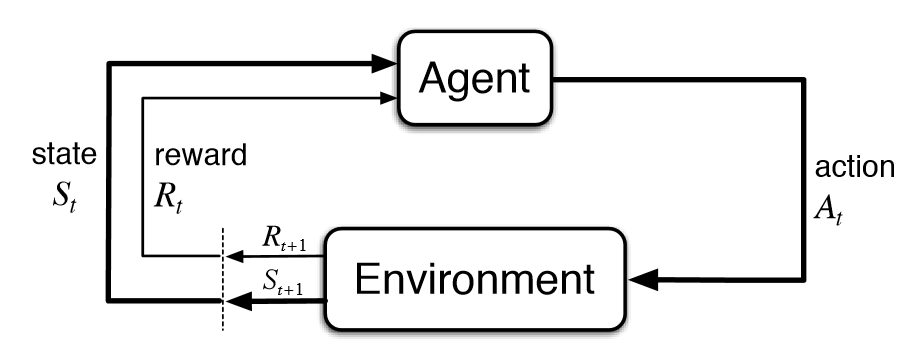
\includegraphics[width=.6\textwidth, height=0.2\textheight]{reinforce.png}
    \caption{Reinforcement Learning Paradigm \cite{sutton_barto_2018}}
    \label{fig:reinforce}
\end{figure}

Reinforcement learning boils down to taking information about an environment and then choosing an action for an agent within the environment that yields the highest reward.  The choices the agent makes is based on the environment and potential future reward. At any point, the environment has some state that contains all of the information about said environment.  Based upon the state of the environment, the agent takes actions and receives a corresponding reward.  Figure \ref{fig:reinforce} shows this process in action. This reward value can be either positive, negative, or zero.  The researcher determines the size of the reward an agent receives based on what the researcher wants the agent to accomplish.  For example, in the game of pong, the agent could receive a positive reward for scoring on the opponent, and a negative reward if scored on.  Since the goal of the agent is to maximize its cumulative reward, it is incentivized to score as much as possible while avoiding being scored on.  

Before moving forward, we should define several key components to creating a reinforcement learning algorithm.  

% Itemized list of defninitons and styling of bullet points
 \renewcommand{\labelitemi}{}
\begin{itemize}

    \item \textit{Agent} - contained within the environment and is what the AI has control over.  The agent performs actions within the environment.
    
    \item \textit{Action} - possible decisions an agent can make in an environment.  For example, an agent playing Pong can either move up or down.  These actions can either be discrete or continuous.
    
    \item \textit{State} - encapsulates all of the information about the environment in a single point in time.  For example, the state for Pong could be the pixel representation of the screen of the game at a given point in time. The screen information for pong contains all of the necessary information that is needed for the agent to make a decision.  It contains the score of each player, the positions of each player, and the location of the ball.
    
    \item \textit{Reward} - an integer value that is given to an agent that is dependent on the state, and the action the agent takes.  It is for the agent to determine whether or not the actions that it is taking is accomplishing the goal it was set out to complete.
    
    \item \textit{Policy} - denoted by $\pi$, the policy determines the actions for the agent in a given state.  In other words, the policy controls the agent’s behavior. It does so by mapping states to actions and choosing actions that yield the highest reward value.
    
    \item \textit{Discount Factor} - denoted by $\gamma$, the discount factor is a value between 0 and 1 that is multiplied by future reward values to reduce the reward given for a given action performed. A discount factor value of 0 means that the future rewards are not considered whatsoever when the agent decides an action, rendering the agent completely shortsighted.  With a discount factor of 1, the agent considers all future actions as heavily as it does current actions, rendering the agent completely far-sighted.  Ultimately, the discount factor is used to control how influential future reward is currently.
    
    \item \textit{Return} - the discounted cumulative reward value.
    
    \item \textit{Value Function} - calculates the return of a policy in a given state.
    
    \item \textit{Q-Value Function} - formally known as the action-value function, the Q-value function is similar to the value function, but with an additional parameter: an action.  The Q-value function computes the return of a policy given a state and an action.
    
    \item \textit{Episode} - a single run of the agent in an environment.  For example, in the game of tic-tac-toe, an episode would consist of each player placing their piece on the board until a player wins or the board is filled.
    
    \item \textit{Trajectory} - denoted by $\tau$, the trajectory is an array containing all of the state, action, and reward values in a given training episode, with each value containing a subscript value denoting the time step.  

\end{itemize}

The decision making process of reinforcement learning can be mathematically described by the Markov Decision Process (MDP) \cite{sutton_barto_2018}. MDPs are mathematical representations of reinforcement learning problems for which precise mathematical statements can be made \cite{sutton_barto_2018}.  All of the definitions defined above are components of MDPs.  MDPs seek to attain an optimal policy that produces the optimal value function, and aim to produce the optimal action-value function.  An important aspect of an environment, which must hold true for an MDP to obtain optimal solutions, is the Markov property. The Markov property states that at any point, the current state must be independent of the past.  In other words, the current state must encapsulate all relevant information for the agent, and does not depend on what happened in previous states.  Anything that has occurred in a previous state can be inferred from information about the current state for the Markov property to hold.

%
% Deep Learning
%
\subsection*{Deep Learning}

Deep learning is a subset of machine learning that uses deep neural networks to recognize patterns and make predictions.  What makes deep neural networks so powerful is that they are universal function approximators, and can be used in a wide variety of scenarios. Deep neural networks have seen many recent breakthroughs in fields such as computer vision, natural language processing, and image recognition.  What separates deep neural networks from regular neural networks is the inclusion of multiple hidden layers. Figure \ref{fig:deep_learning} shows the similarities and differences between the architectures of a simple neural network and a deep neural network.


% Deep Learning Figure - Simple VS Deep
\begin{figure} [ht!]
    \centering
    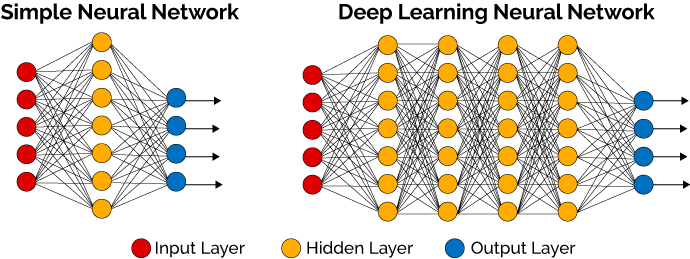
\includegraphics[width=1\textwidth, height=0.2\textheight]{deepLearning.png}
    \caption{Architecture of a Deep Learning Network \cite{iesc_2018}}
    \label{fig:deep_learning}
\end{figure}

The idea behind deep learning is to extract multiple levels of representation from a given data set to allow for more robust and complex approximations \cite{lecun_2015}. Deep neural networks are made up of vertices, called neurons, and are connected by weighted edges that take numerical data.  The initial layer, known as the input layer, takes in data that is then passed to the first hidden layer.  At every hidden layer, the data coming from the previous layer is multiplied by a weight, and summed.  A value known as a bias is then added to the sum. The bias helps to shift the activation function to better fit the data \cite{collis_collis_2017}. Before the layer generates its output, an activation function is applied.  Figure \ref{fig:activation} shows the process of taking input and generating output. The activation function, along with the bias, help to calculate the optimal approximation.  

Typically, there are two phases for developing a deep neural network: training, and evaluation.  The training phase involves feeding the neural network data to learn from, and then optimizing the neural network periodically.  In the case of supervised learning, it is during training phase  an error value is computed.  This error value is also known as the loss, and different loss functions can be applied to compute the loss.  Essentially, the loss value takes the output of the neural network, and subtracts it from the expected output.  The loss value is typically squared  so that the loss is always non-negative.  After the loss has been computed, backward propagation of the error occurs.  This is the training process as this is where the learning takes place.  To modify the model’s weights such that they minimize the amount of computed loss, the model must know how the weights need to be adjusted.  This is done by taking the gradient of the neural network. Figure \ref{fig:gradient} shows a 3D representation of a gradient vector. The value of the weights are then adjusted so that the output of the model is more accurate.  

% Anatomy of a neural network node
\begin{figure} [h!]
    \centering
    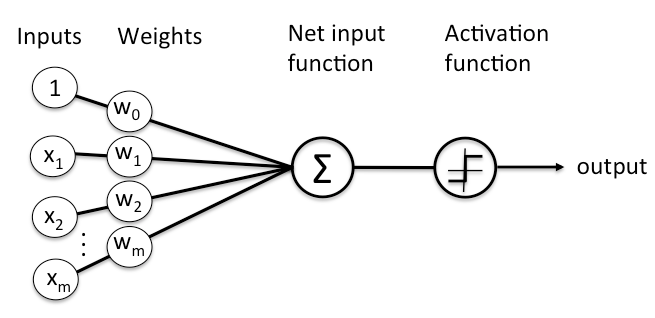
\includegraphics[width=.7\textwidth, height=0.2\textheight]{activation.png}
    \caption{Anatomy of a Neural Network Node \cite{skymind}}
    \label{fig:activation}
\end{figure}


The gradient tells the model what the slope of our loss function is, helping us to adjust our parameters in the direction that best minimizes the loss.  The size of the parameter update is controlled by the learning rate, denoted by $\alpha$.  The value of the learning rate is typically between 0 and 1, and varies based on the rate of convergence to the optimal solution.  If the learning rate is too high, the weights can be adjusted too much and overshoot the correct solution.  This could potentially lead to divergence and the model never learns the optimal solution that minimizes the loss.  Conversely, if the learning rate is too low, it could take a long time to converge to the optimal solution.  The figure \ref{fig:gradient} represents the gradient of some cost function, $J(w,b)$.  The x and z axis denotes the values of the parameters $w$ and $b$.  The arrow at the bottom corresponds to the values for parameters $w$ and $b$ such that they minimize the amount of loss generated the by the model.

\begin{figure} [ht!]
    \centering
    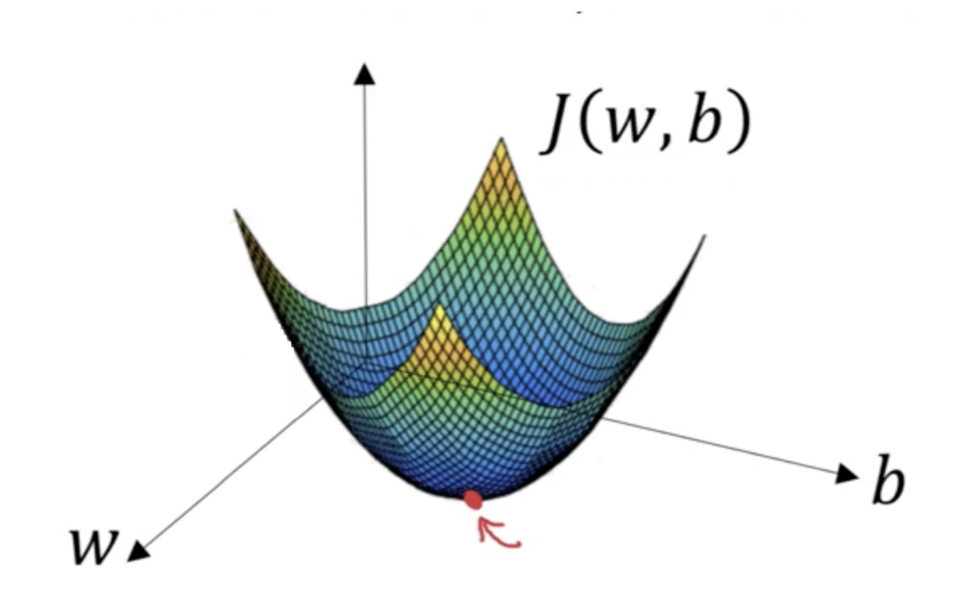
\includegraphics[width=.8\textwidth, height=0.3\textheight]{gradient.png}
    \caption{Gradient of the Neural Network \cite{donges_donges_2018}}
    \label{fig:gradient}
\end{figure}

After the model is done training, it is then evaluated on an entirely different data set from what it was trained on.  The model’s weights are now static, and the results are evaluated to see how it handles input that it has not worked with before.    

%
% Convolutional Neural Networks
%
\subsection*{Convolutional Neural Networks}
Convolutional neural networks work like regular neural networks, but work well with extracting features from image data.  Convolutional neural networks are capable of taking images as input and extracting spatial and temporal dependencies of an image \cite{saha_saha_2018} .

%
% Deep Learning with Reinforcement Learning
%
\subsection*{Deep Learning with Reinforcement Learning}

There are difficulties reinforcement learning algorithms, though.  For example, with the Q-learning algorithm, it must maintain a matrix that contains all of the possible state-action pair values.  In environments with a continuous state space and/or a continuous action space, it becomes impossible to track the action-value for all actions in all states.  More specifically, this function is called the action-value function or Q-value function.  This function can be approximated by using deep neural networks.  This is how the Deep-Q network (DQN) developed by DeepMind handles the issue of arbitrarily large state-action spaces.  

%
% Starcrat II
%
\subsection*{Starcraft II}

StarCraft II is a real-time strategy game (RTS) that is known for its competitive scene and steep learning curve.  RTS’s are games in which the player manages a vast army of units, as opposed to a single unit.  In StarCraft II, the player is responsible for collecting resources, creating structures, manufacturing units, attacking and defending structures, investing in technological advancements, and much more.  The game is also known for its fast pace; the in-game time is sped up to 1.4 times normal time.  This means that a minute of game time is only 42 seconds in real time.  Because of this fast-paced and complex nature, researchers have been interested in developing AIs to compete against the best human Starcraft II players.

Video games serve as fantastic environments for implementing and testing reinforcement learning algorithms.  They allow for environments in which researchers have fine grained control of the environment, and relevant environment data is readily available. Starcraft II is no exception, and its environment is excellent for AI research.

%
% PySC2 Library
%
\subsection*{PySC2 Library}
The PySC2 library is a set of tools that is used to access the StarCraft II Machine Learning API built by Blizzard Entertainment. The original API is based on C++ code that is deeply linked within the SC2 engine itself and allows for the access of scripted bots, machine-learning based bots, and replay analysis within the SC2 environment. The role of PySC2 was to give access to this API, allowing for python based reinforcement learning environment. PySC2 enabled allows users to create agents in python that can gather observations and perform actions within the game. 

%
% Deepmind Starcraft II mini games
%
\subsection*{DeepMind StarCraft II Mini-games}

% Minigame 
\begin{figure} [ht!]
    \centering
    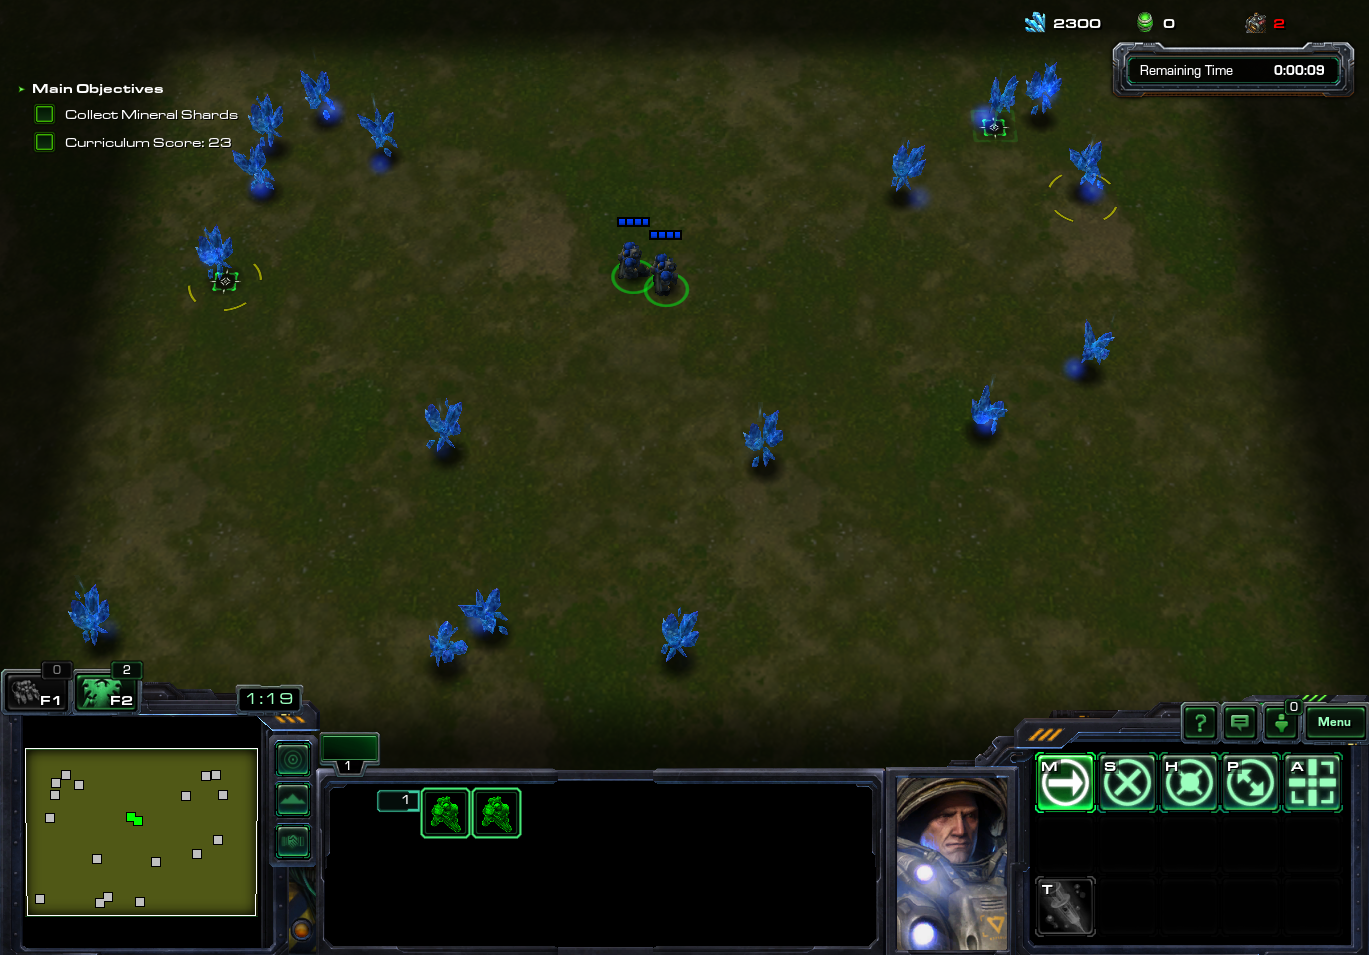
\includegraphics[width=.6\textwidth, height=.3\textheight]{Game.png}
    \caption{Mineral collection mini-game}
    \label{fig:minigame}
\end{figure}

Within the StarCraft II environment is the ability to develop intricate custom maps and game modes that players can develop. This allows for the creation of mini-games within the StarCraft II environment using the large library of units, maps, and functions that are provided by the game. 

There are two major benefits to using the PySC2 library: the user can access the current state of the Starcraft II environment and the user can choose from a list of pre-built mini-games that can be played by an AI created by the user. The mini-game that we chose was the mineral collection game because of its fast pace, and clear goal. These conditions made it simple to define the reward for our AI. The Agent controls actors within the map to collect minerals, and it receives a score based on the number of minerals collected within the given time frame of one minute and thirty seconds. Figure \ref{fig:minigame} shows the mini-game being played by the AI during an episode. If the Agent collects all twenty of the generated minerals before one minute and thirty seconds have passed, the map resets and generates new locations for minerals to be collected. The minerals generated by the map are random and will change their positions after a reset, even if this reset happens before an episode completes.

%
% Map Customization (NOT NEEDED IN PAPER BECASE WE USED RANDOM MAPS!)
%
%\subsection*{Map Customization}
%The random nature of the minerals within the mini-game made it difficult to observe improvements in the AI, because it could seem like it’s improving if  it had favorable random mineral replacement. So, the mini-game was modified to use static mineral placements that would not renew if all minerals were collected. This allowed the AI to run more episodes in a controlled environment so that randomness did not affect the reward and allowed it to improve on already established knowledge. 

%%%%%%%%
%SECTION - Methodology
%%%%%%%%
\section*{\Large Methodology}

%
% Background of meothodology?
%
\subsection*{Initial Preparation}

We used the Python programming language to create our model and experiment.  We also used the Pytorch library to create our convolutional neural networks, and to implement our reinforcement learning algorithms.

%
% Deep Neural Network Setup
%
\subsection*{Deep Neural Network Setup}

We developed a deep convolutional neural network to approximate our policy function. Our neural network has three hidden layers, all of which are convolutional layers that are batch normalized.  The activation function for each of our hidden layers is the ReLU activation function. The output layer is a softmax layer with 21 output neurons.

%
% REINFORCE algorithm (NOT DONE HERE!)
%
\subsection*{REINFORCE Algorithm}

The REINFORCE algorithm is a policy gradient algorithm that increases the probabilities of taking actions that lead to a higher return value. Additionally, it decreases the probability of taking an action that leads to a lower return value until you arrive at the optimal policy.  The REINFORCE algorithm is an on-policy algorithm, meaning the policy is directly evaluated and improved. This is opposed to calculating the optimal Q-value for every given state and then creating a policy based on these values.  In the latter case, this would be known as off-policy learning. The algorithm works by first sampling trajectories by running the policy, and computing the policy loss by multiplying the negative log probability of taking each action in the episode by the return at each time step.

%
% System Setup
%
\subsection*{System Setup}

The system that was used to run the simulations contained an Intel i7-8700k CPU and Nvidia GTX 1080 Ti graphics card. The use of Nvidia CUDA was an important part of the system set up for use with our AI. CUDA is a parallel computing library that allows a graphics processing unit (GPU) to be used as a general processor. This can be beneficial for a program that requires a large amount of algebraic and geometric calculations because GPUs excel at performing these types of calculations. Using the CUDA library, the AI was ran exclusively on the Nvidia GTX 1080 Ti graphics card, allowing our algebra based algorithm to compute efficiently. 


%
% Experimental Setup
%
\subsection*{Experimental Setup}

% Agent seeing? Visual 
\begin{figure} [h]
    \centering
    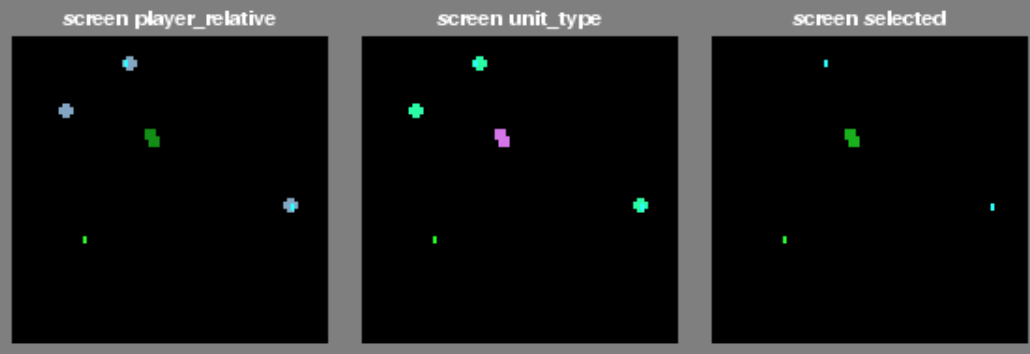
\includegraphics[width=1\textwidth, height=0.2\textheight]{screen.png}
    \caption{What the Agent is 'Seeing'}
    \label{fig:game_screen}
\end{figure}

For our experiments, we needed a way to determine how our agents should perform actions.  To do this, we decided to use a discrete action space for our AI.  The standard mineral collection mini-game has 20 minerals placed randomly on the map, and the agent’s actions correspond to the Cartesian coordinates of the minerals with respect to the marines.  The actions are in order from the closest mineral to the furthest mineral. Since the mini-game has two marines, we simplified the process by treating the two marines as a single unit.  To compute the coordinates, we use the average distance between the two marines as the the starting point.  We then compute the euclidean distance from the marines to each mineral so that we can determine the order of the actions.  We then add an additional action that corresponds to a no operation action.  This is to give the agent the option to not have to change where it is going if it sees no reason to.  In all, our agent has in total 21 actions, and the output of our convolutional neural network is a tensor with 21 values.  The values of the output tensor are the probabilities of taking each action.  If an agent collects a mineral, that action is replaced with a no operation action.  No operation actions are sorted at the bottom of the list.

For the input of our neural network, the PySC2 library exposes feature layers to the user.  The feature layers are preprocessed images of the mini-map and the screen.  We use three different representations of the screen as the input to our neural network.  The feature screens we used were the player\_relative, unit\_type, and selected screens.  The player\_relative feature screen represents the alliances of the units with respect to the player.  Green represents the player, light blue represents neutral units, and red represents enemies.  The unit\_type feature screen represents the types of each unit on the screen. The screen selected represents the selected units and the select box the AI makes. Figure \ref{fig:game_screen} shows a visual representation of the feature screens.

%%%%%%%%
%SECTION - Results
%%%%%%%%
\section*{\Large Results}

Our results are extensive, yet preliminary. Figure \ref{fig:test1} corresponds to the return the agent received after each episode.  The agent ran in total for 8,000 episodes. The agent's return values oscillated quite frequently. At points the model performed very well, but never seemed to play consistently. There are many potential reasons for this. First, we simply might not have trained the model enough. In the paper created by DeepMind on the PySC2 library, they conducted reinforcement learning experiments, and the number of episodes that were completed were far more than we had done. 

% Rewards figure
\begin{figure} [H]
    \centering
    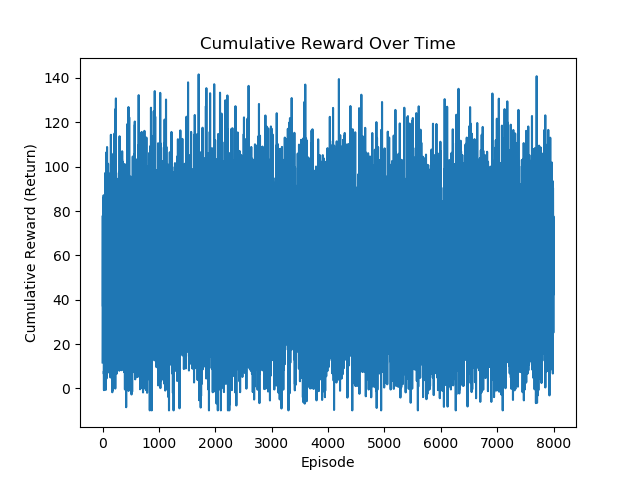
\includegraphics[width=.75\textwidth, height=.4\textheight]{rewardLine.png}
    \caption{The results of our experiments}
    \label{fig:test1}
\end{figure}



On the x-axis of Figure \ref{fig:test2}, the values correspond to the number of game steps as opposed to the number of episodes. A game step is a single action, and for the mineral collection mini-game, each episode has 480 game steps.  If we divide the total number of game steps by the number of game steps per episode, we get $\frac{600,000,000}{480} = 1,250,000 $ episodes.  In comparison, we only ran 8,000 episodes.  The lack of training time did not allow for the model to converge to the optimal solution for the mineral collection mini-game.  We simply did not have the resources to compute that many episodes in a reasonable amount of time.  We ran the training session for approximately 72 hours to complete 8,000 episodes.  Due to hardware limitations, we could not run 10,000+ episodes in a reasonable amount of time.  

%Figure from Deep Mind SC2 AI
\begin{figure} [ht!]
    \centering
    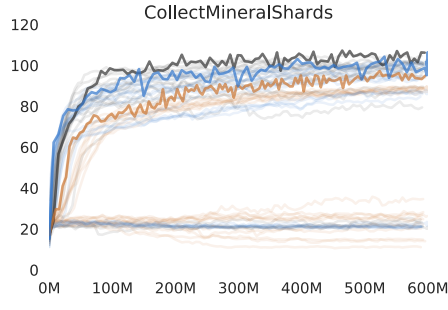
\includegraphics[width=.75\textwidth, height=.4\textheight]{deepmindresults.png}
    \caption{DeepMind's test results \cite{Vinyals2017StarCraftIA}}
    \label{fig:test2}
\end{figure}

Another weakness of our model was that it could have been more robust.  A more robust neural network architecture would involve the use of recurrent neural networks (RNN). These neural networks are able to keep track of time, and they work well with sequences. In the DeepMind paper, they created Long-Short Term Memory (LSTM) recurrent neural networks. LSTM is a popular RNN architecture that is typically used with time series data \cite{Vinyals2017StarCraftIA}.

%%%%%%%%
%SECTION - Discussion
%%%%%%%%
\section*{\Large Discussion}

%
% Personal reaction to project
%
\subsection*{Our Feelings About This Project}

The reinforcement learning research project was both challenging and rewarding.  There were many theoretical concepts that we had to first comprehend before we could even begin. Also, we had to learn how we could go about building an AI. We studied the first few chapters of Reinforcement Learning: An Introduction by Sutton and Barto \cite{sutton_barto_2018} to develop a theoretical basis of reinforcement learning concepts before constructing our AI. Researching a framework that would work for us was also something we struggled with. There was very limited documentation of the PySC2 library, making it challenging to create our AI.  We had to scour through the GitHub repository, and dig through the source code to figure out how certain aspects of the library worked. Although this project was quite difficult, we are very happy we had the opportunity to learn more about how reinforcement learning works, and we are pleased to have been able to implement a deep reinforcement learning algorithm.\newpage  

%
% Classroom Takeaway
%
\subsection*{Classroom Takeaway - Expansion Into Course}

This project could be modified into a curriculum for a semester long class by splitting up the parts of the experiment into milestones that students could reach. In the beginning, students could study the theoretical concepts of reinforcement learning while starting to develop a notion of what kind of mini-game they would implement. Moving forward, they could be guided into building their first simple neural network. This will help to solidify the students understanding about the algorithms by implementing them. During this time they could familiarize themselves with the SC2 map editor program to find out about how the internals of the provided mini-games function. 

Once students have established the foundation of what they need to know, they could be split into groups that will last for the rest of the semester. After establishing these groups, students would then begin to experiment with the PySC2 library. Working together, they could complete small assignments, such as creating their own custom maps, to help familiarize themselves with the library. Once the students have become comfortable working with the library and their groups, they would submit a proposal. This proposal would include what they would like their AI agent to do along with reasonable milestones to complete along the way. The rest of the semester would be a guided learning experience where the students work together in their teams while the professor would assist them in any serious roadblocks that they encounter.

This idea of a guided learning experience through this course will not only help the students learn about the foundations of reinforcement learning algorithms, it will also help give them a sense of how to conduct research on their own. Naturally, the professor will be there to assist them, but they are handed this library to use and allowed to decide among themselves what they want their agent to achieve. It is extremely important for programmers to be able to discover new things on their own, and this is an excellent way to lightly guide the students into these skills.  


\subsection*{Conclusion}
Through employing deep reinforcement learning algorithms, we managed to successfully create an deep learning AI agent. Based upon other research on reinforcement learning agents \cite{Vinyals2017StarCraftIA}, it could take thousands of more episodes before our AI converges towards maximum efficiency. Our model was able to take screen data as input, and convert that into an action. The model's improvement didn't converge, but there were several occasions where the model performed well.  Regardless of the results, we are all appreciative of the opportunity to learn about deep reinforcement learning throughout the process of creating an AI.

\newpage
\bibliographystyle{IEEEtran}
\bibliography{refs.bib}


\end{document}
